\definecolor{cardboard}{RGB}{192,143,79}

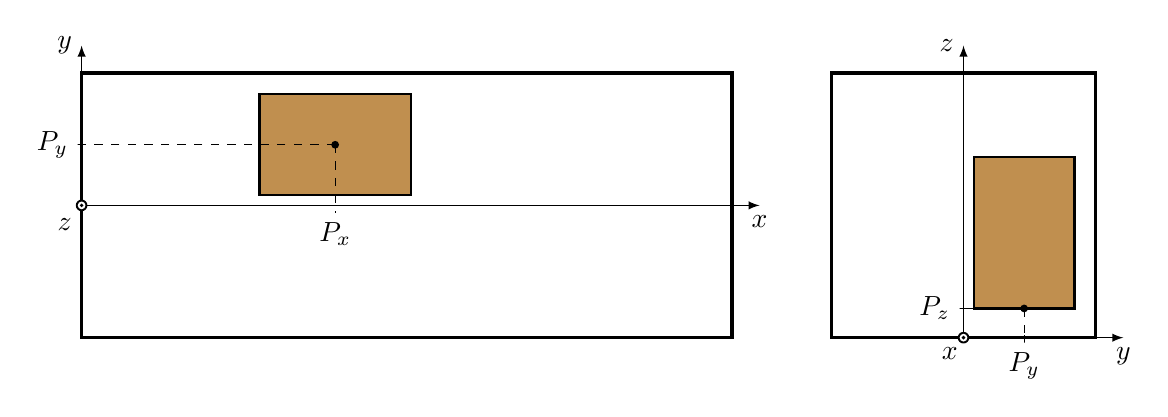
\begin{tikzpicture}[
	scale=0.7
	]
	
	\draw [->, >=latex] (0, 0) -- (12.3cm, 0) node [anchor=north] {$x$};
	\draw [->, >=latex] (0, 0) -- (0, 2.9cm) node [anchor=east] {$y$};
 	\node (pallet) at (4.6, 1.1) [draw, thick, scale=0.8, fill = cardboard, minimum width=2.4cm,minimum height=1.6cm] {};
 	\fill (4.6, 1.1) circle (2pt)  coordinate (center);
 	\draw [dashed] (center) --++ (0, -1.1) --++ (0, -4pt)  node [anchor=north] {$P_x$};
 	\draw [dashed] (center) --++ (-4.6, 0) coordinate (y);
 	\draw (y) --++ (-2pt, 0) node [anchor=east] {$P_y$} --++ (4pt, 0) ;
	\draw [very thick] (0, -2.4) rectangle (11.8, 2.4);
	\fill (0, 0) circle (3pt) node [anchor=east, yshift = -7pt] {$z$};
	\fill [color = white](0, 0) circle (2pt);
	\fill (0, 0) circle (1pt);
	
	\draw [->, >=latex] (16, -2.4) -- (18.9, -2.4) node [anchor=north] {$y$};
	\draw [->, >=latex] (16, -2.4) -- (16, 2.9) node [anchor=east] {$z$};

 	\node (pallet) at (17.1, -0.5) [draw, thick, scale=0.8, fill = cardboard, minimum width=1.6cm,minimum height=2.4cm] {};
  	\fill (17.1, -1.87) circle (2pt)  coordinate (center);
 	\draw [dashed] (center) --++ (0, -0.55) coordinate(y);
 	\draw (y)--++ (0, -2pt) node [anchor=north] {$P_y$} --++ (0, 4pt);
 	\draw [dashed] (center) --++ (-1.1, 0) coordinate (z);
 	\draw (z) --++ (-2pt, 0) node [anchor=east] {$P_z$} --++ (4pt, 0) ;
	\draw [very thick] (13.6,  -2.4) rectangle (18.4, 2.4);
	\fill (16, -2.4) circle (3pt) node [anchor=north, xshift = -5pt] {$x$};
	\fill [color = white](16, -2.4) circle (2pt);
	\fill (16, -2.4) circle (1pt);
\end{tikzpicture}
